\documentclass{standalone}
\usepackage{tikz, xcolor, amsmath}
\newcommand*\circled[1]{\tikz[baseline=(char.base)]{
            \node[shape=circle,draw,inner sep=2pt] (char) {#1};}}
%% Couleurs %%
\usepackage{xcolor}
\definecolor{bleu}{RGB}{14, 68, 175}
\definecolor{BGbleu}{RGB}{222, 233, 255 }
\definecolor{BGorange}{RGB}{255, 216, 154}
\definecolor{rouge}{RGB}{201, 0, 0}
\definecolor{vert}{RGB}{14, 137, 0}
\definecolor{BGgris}{RGB}{222,230,230}
\newcommand\rouge[1] {{\color{rouge}{#1}}}
\newcommand\bleu[1] {{\color{bleu}{#1}}}
\newcommand\green[1]{{\color{vert}{#1}}}

\begin{document}
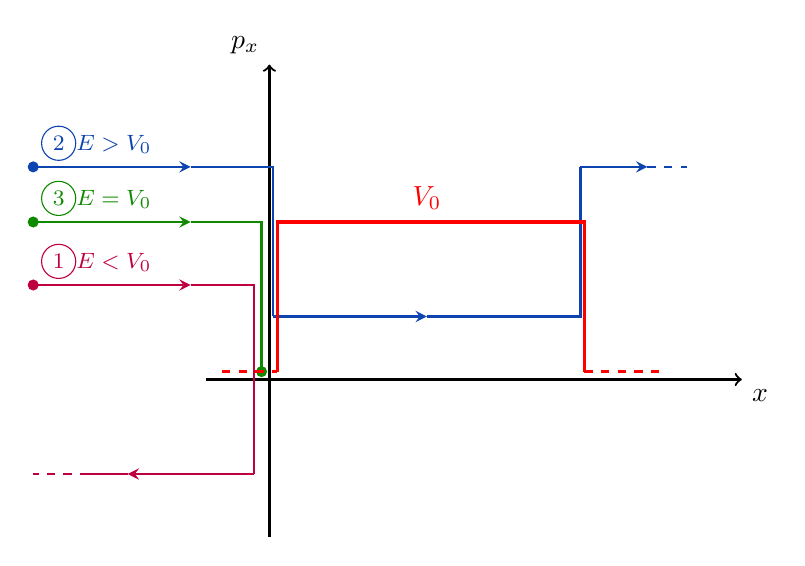
\begin{tikzpicture}
    \draw[thick, ->] (-0.8,0) -- (6,0) node[below right] {$x$} ;
    \draw[thick, ->] (0,-2) -- (0,4) node [above left]{$p_x$};

    
    % Flèche particule qui arrive avec une faible énergie
    \node at (-2.2, 1.5) {\footnotesize {\color{purple}{\circled{1}$E < V_0$}}} ;
    \fill[purple] (-3, 1.2) circle(2pt) ;
    \draw[thick, purple, -stealth] (-3, 1.2) -- (-1, 1.2) ;
    \draw[thick, purple] (-1, 1.2) -- (-0.2, 1.2) -- (-0.2, -1.2);
    \draw[thick, purple, -stealth] (-0.2, -1.2) -- (-1.8, -1.2) ;
    \draw[thick, purple] (-1.8, -1.2) -- (-2.3, -1.2) ;
    \draw[thick, purple, dashed] (-2.3, -1.2) -- (-3, -1.2) ;
    
    % Flèche particule qui arrive avec une plus grande énergie
    \node at (-2.2, 3) {\footnotesize {\color{bleu}{\circled{2}$E > V_0$}}} ;
    \fill[bleu] (-3, 2.7) circle(2pt) ;
    \draw[thick, bleu, -stealth] (-3, 2.7) -- (-1, 2.7) ;
    \draw[thick, bleu] (-1, 2.7) -- (0.05, 2.7) -- (0.05, 0.8);
    \draw[thick, bleu, -stealth] (0.05, 0.8) -- (2, 0.8);
    \draw[thick, bleu] (2, 0.8) -- (3.95, 0.8)  -- (3.95, 2.7);
    \draw[thick, bleu, -stealth] (3.95, 2.7) -- (4.8, 2.7) ;
    \draw[thick, bleu, dashed] (4.8, 2.7) -- (5.3, 2.7) ;
    
    % Flèche particule qui arrive avec une énergie égale
    \node at (-2.2, 2.3) {\footnotesize {\color{vert}{\circled{3}$E = V_0$}}} ;
    \fill[vert] (-3, 2) circle(2pt) ;
    \draw[thick, vert, -stealth] (-3, 2) -- (-1, 2) ;
    \draw[thick, vert] (-1, 2) -- (-0.1, 2) -- (-0.1, 0.1);   
    \fill[vert] (-0.1, 0.1) circle(2pt) ;
    
    % Potentiel
    \draw[very thick, red] (0.1, 0.1) -- (0.1, 2) -- (4, 2) -- (4, 0.1) ;
    \draw[very thick, red, dashed] (-0.6, 0.1) -- (0.1, 0.1) ;
    \draw[very thick, red, dashed] (4, 0.1) -- (5, 0.1) ;
    \node at (2, 2.3) {{\color{red}{$V_0$}}} ;
\end{tikzpicture}
\end{document}